\chapter{相關研究}
{透過使用者之網頁瀏覽歷史紀錄預測使用者性格特質之應用極為廣泛,本章節將透過生活中較常接觸之應用以及具有較高影響力之應用來介紹。}

\section{網頁瀏覽紀錄之分析應用}
{
利用使用者之網頁瀏覽紀錄來決定投放廣告之內容逐漸成為目前網頁廣告之趨勢,透過使用者近期瀏覽過的網頁能夠較為了解此使用者目前對於何種議題以及商品有興趣,找出對應之商品廣告進行投放是目前最能夠打動使用者之消費欲望的方法之一,以上之廣告策略稱之為個人化廣告。\par

而在眾多廣告投放平台中又以 Google 成立的廣告計劃 Google AdSense 所提供的個人化廣告~\cite{merriman1999method}最為廣泛,其原因在於大部分的使用者以 Google Chrome 瀏覽器進行網頁瀏覽,而使用者通常會以 Google Gmail 之帳號登入 Chrome 來獲取平時習慣使用的設定,包括各網站之會員帳號密碼等資訊,而個人化廣告設定在 Chrome 中預設是開啟狀態,因此在登入 Google 帳號的同時,會將此瀏覽器之 cookie 傳送至 Google 之資料中心進行分析, Google 藉此能夠了解此使用者最近搜尋的關鍵字與網站瀏覽紀錄資訊進行最適合的廣告投放效果,此網頁瀏覽紀錄分析之應用是我認為是目前生活中最常見的應用之一。此應用為透過使用者跨網頁的瀏覽紀錄預測 “ 使用者對何種廣告較有興趣 ”,而本篇論文則是透過使用者跨網頁的瀏覽紀錄預測 “ 使用者的個人資訊以及大六性格特質分數 ”。\par
\clearpage

另一方面,網頁瀏覽記錄同時也包含使用者在特定網頁平台上所進行之瀏覽行為記錄。其中我認為日常生活中較為頻繁接觸的電子商務類型網頁之感受最為強烈,其中以 {\se Amazon.com} 為例,使用者在電子購物平台中所瀏覽的商品與購物清單之紀錄都被 Amazon 紀錄下來~\cite{freno2015one},因此商品推薦列表(圖 ~\ref{fig:rec_list})中時常包含了使用者感興趣的元素。此應用為透過使用者在 “ 特定網頁平台 ” 內商品的瀏覽行為預測使用者對於何種商品較有興趣,而本篇論文則是透過使用者 “ 跨網頁 ” 的瀏覽資訊進行使用者相關資訊的預測。

}

\begin{figure}
    \graphicspath{{fig/}}
    \begin{center}
    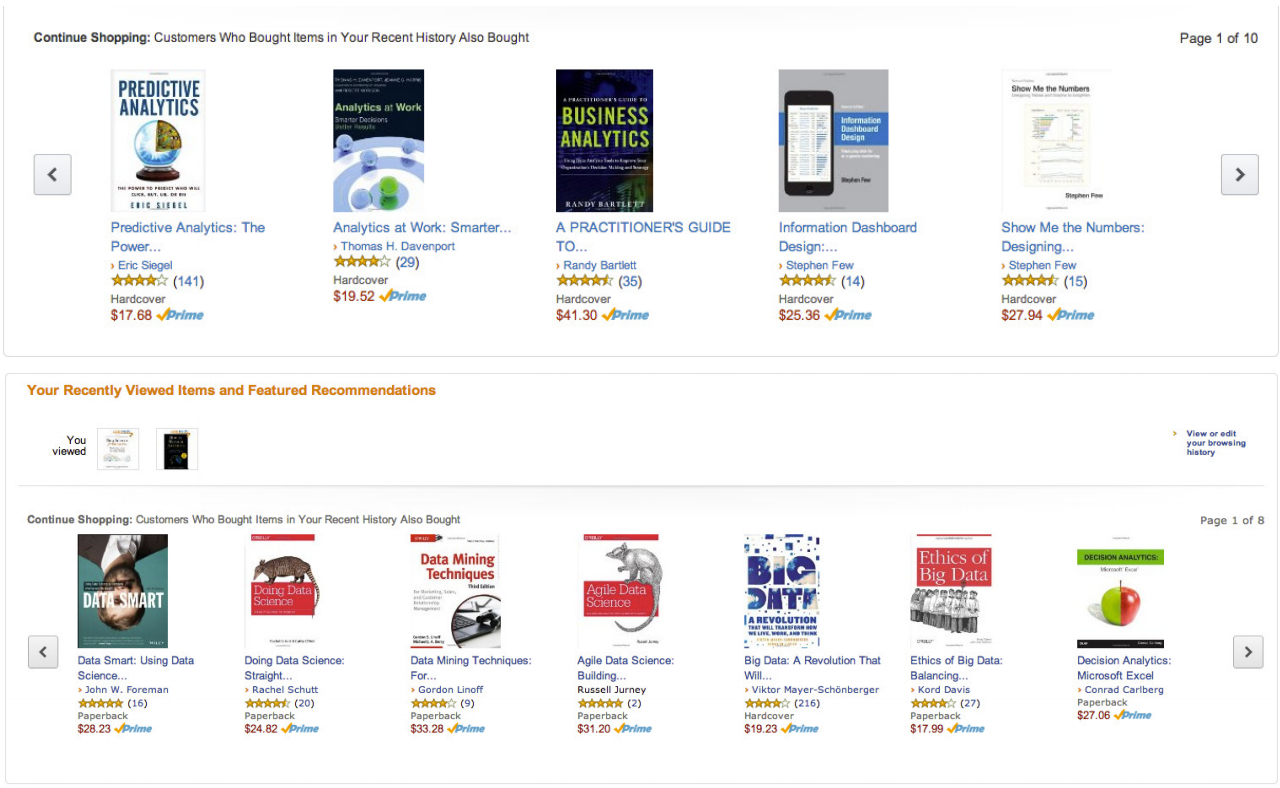
\includegraphics[width=\linewidth]{rec_list.png}
    \caption{{\se Amazon.com} 中使用者之根據購買紀錄進行推薦之商品清單(上方),以及根據使用者目前之瀏覽紀錄進行推薦之商品清單(下方)}
    \label{fig:rec_list}
    \end{center}
\end{figure}

\section{根據使用者之性格特質給予特定廣告之策略}
{Facebook 是目前最受歡迎的社群平台之一,同時大部分的使用者在 Facebook 上留下了許多個人資訊,本段對於個人資訊之定義為使用者對於何種文章類型(體育、音樂、書籍、餐廳等)表示喜歡(Like)。藉由分析使用者之個人資訊,預測使用者之年齡、性別、職業甚至是個性~\cite{kosinski2013private},進而根據不同個性之使用者投放特定廣告~\cite{matz2017psychological},是目前 Facebook 在選擇投放廣告對象之依據方法之一。此應用為透過使用者在 “ 特定網頁平台內 ” 對何種文章表示喜歡來進行大五性格特質分數的預測,而本篇論文則是透過 “ 跨網頁 ” 的瀏覽紀錄預測使用者的個人資訊以及大六性格特質分數。\par

 
針對不同性格特質給予廣告之實際影響甚至可以追朔至 $2016$ 年美國總統選舉,根據媒體報導劍橋分析公司(Cambridge Analytica)透過社群平台 Facebook 取得了 $5,000$ 萬名使用者之個人資訊~\cite{cadwalladr2018revealed}進行使用者性格特質之預測,再針對不同性格特質之使用者投放競選廣告而影響選情。縱使報導的真實性尚未確定,但是對特定性格之使用者投放特定廣告之影響力已經被證實~\cite{cadwalladr2018revealed}。

}

\section{預測使用者在特殊節日之網頁瀏覽行為變化}
{
基於我先前之研究~\cite{lien2017taai},透過與本論文相同的資料集,分析使用者在特殊節日期間與平時對於電子商務平台相關網頁瀏覽比例之比較,以使用者瀏覽網頁的種類以及使用者之性別、年齡、感情狀態當作特徵,藉由基本的監督式學習模型(K-nearest neighbors, Support vector machine, Random forest and Logistic regression) 預測使用者在特殊節日是否會提高瀏覽電子商務平台網頁之比例,例如:中秋節、單身節以及聖誕節,其預測結果如表~\ref{tab:classifier-auc}。\par

\begin{table}[tbh]
\centering
\caption{四種分類器預測結果之 AUCs 比較}
\label{tab:classifier-auc}
\begin{tabular}{c|c|c|c|c|c|c}
\hline
    & \multicolumn{2}{c|}{Moon Festival} & \multicolumn{2}{c|}{Singles Day} & \multicolumn{2}{c}{Christmas} \\ \hline\hline
    & Training & Test & Training & Test & Training & Test \\ \hline
KNN & 0.71     & 0.55 & 0.75     & 0.63 & 0.78     & 0.72 \\ \hline
LR  & 0.73     & \textbf{0.65} & 0.70     & 0.61 & 0.82     & 0.73 \\ \hline
SVM & 0.74     & 0.64 & 0.84     & \textbf{0.64} & 0.84     & \textbf{0.77} \\ \hline
RF  & 0.99     & 0.60 & 0.99     & 0.60 & 0.99     & 0.68 \\ \hline
\end{tabular}
\end{table}


基於此研究結果,我認為此研究透過使用者之網頁瀏覽歷史紀錄之應用能夠幫助電子商務平台針對不同瀏覽習慣之使用者給予特定的市場行銷手段,能夠節省廣告成本並使廣告效果最大化。
}
